%\documentclass[11pt]{article}
\documentclass[answers]{exam}

\usepackage{amsmath}
%\usepackage{extsizes}
\usepackage{amsmath,amssymb}
%\usepackage{omegavn,ocmrvn}
%\usepackage[utf8x]{inputenc}
\usepackage[utf8]{vietnam}
\DeclareUnicodeCharacter{00A0}{ }

\usepackage{longtable}
\usepackage{answers}
\usepackage{graphicx}
\usepackage{array}
\usepackage{pifont}
\usepackage{picinpar}
\usepackage{enumerate}
\usepackage[top=3.0cm, bottom=3.5cm, left=3.5cm, right=2.5cm] {geometry}
\usepackage{hyperref}


\newtheorem{bt}{Câu}
\newcommand{\RR}{\mathbb R}
\Newassociation{sol}{Solution}{ans}
\newtheorem{ex}{Câu}
\renewcommand{\solutionstyle}[1]{\textbf{ #1}.}


\begin{document}
% \noindent
\begin{tabular*}
{\linewidth}{c>{\centering\hspace{0pt}} p{.7\textwidth}}
Trường ĐHKHTN, ĐHQGHN & {\bf Học Kỳ 2 (2019-2020)}
\tabularnewline
K61 TTƯD \\ Lớp thầy Hà Phi & {\bf Giải Tích Số 2 (MATLAB)}
\tabularnewline
\rule{1in}{1pt}  \small  & \rule{2in}{1pt} %(Due date:)
\tabularnewline

%  \tabularnewline
%  &(Đề thi có 1 trang)
\end{tabular*}
%

\begin{center}
NO 1: GIẢI PHƯƠNG TRÌNH VÀ HỆ PHI TUYẾN \\ GIÁO TRÌNH QUARTERONI, 3 ED.
\end{center}

%\Opensolutionfile{ans}[ans1]
\printanswers

\begin{bt} (Bài toán đầu tư) Vào đầu mỗi năm một khách hàng đầu tư $v$ Euro vào một tài khoản tiết kiệm, và sau $n$ năm rút ra được tổng cộng $M$ Euro. Ta muốn tính lãi suất trung bình $r$ của việc đầu tư này.
Khi đó $M$ và $r$ được liên kết với nhau bởi phương trình 
%
\[
M = v \sum_{k=1}^{n} (1+r)^k = v \dfrac{1+r}{r} \Big[ (1+r)^n - 1 \Big].
\]
%
Do đó $r$ chính là nghiệm của phương trình $f(r)=0$, với $f(r) := M -  v \dfrac{1+r}{r} \Big[ (1+r)^n - 1 \Big]$.\\
Áp dụng: Bài tập 2.13 (trang 73)	
\end{bt}

\begin{bt} (Phương trình trạng thái của khí ga) Chúng ta muốn xác định thể tích $V$ của một khối khí ga tại nhiệt độ $T$ và áp suất $p$. Phương trình trạng thái là
	%
	\[
	\Big[ p + a (N/V)^2 \Big] \ (V-Nb) = k \ N \ T.
	\]
	%
	trong đó $a$ và $b$ là hai hệ số của khí ga (phụ thuộc vào đặc tính của mỗi loại khí ga), $N$ là số các phân tử được chứa trong thể tích $V$ và $k$ là hằng số Boltzmann. Do đó $V$ chính là nghiệm cảu một phương trình phi tuyến.\\
	Áp dụng: Bài tập 2.2 (trang 72)	
\end{bt}

\begin{bt} (Hệ thống thanh) Một hệ cơ khí được biểu diễn bởi 4 thanh cứng như trong hình vẽ \ref{fig:lec11}. 
	\begin{figure}[!h]
		\centering
		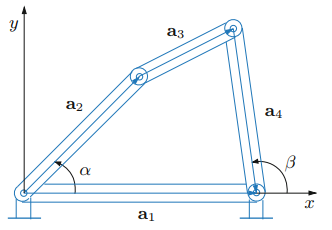
\includegraphics[width=0.3\linewidth]{Lec1_1.png}
		\caption{Hệ cơ khí bao gồm 4 thanh cứng}
		\label{fig:lec11}
	\end{figure}	
Với một giá trị (chấp nhận được) của góc $\beta$, chúng ta xác định giá trị của góc $\alpha$. Bằng việc sử dụng đẳng thức vector
%
\[
a_1 - a_2 - a_3 -a_4 = 0
\]
%
ta thu được mối liên hệ giữa 2 góc (thường được gọi là phương trình Freudenstein)
%
\[
\dfrac{a_1}{a_2} \cos(\beta) - \dfrac{a_1}{a_4} \cos(\alpha) - \cos(\beta - \alpha) =  - \dfrac{a_1^2 + a_2^2 - a_3^2 + a_4^2}{2 a_2 a_4} \ .
\]
%
Đây là phương trình phi tuyến của biến số $\alpha$, và nó chỉ có nghiệm với một số giá trị của $\beta$. Phương trình này có thể có nhiều hơn 1 nghiệm hoặc vô nghiệm. \\
Áp dụng: Bài tập 2.9 (trang 73)	
\end{bt}

\begin{bt} (Mô hình dân số) Trong quá trình nghiên cứu sự phát triển cư dân của một loài (hoặc chủng virus), phương trình $x^+ = \phi(x) = xR(x)$ biểu diễn mối liên hệ giữa số cá thể ở thế hệ $x$ và số cá thể ở thế hệ tiếp theo. 
	Hàm số $R(x)$ mô hình tốc độ biến đổi của loài đang xét và có thể được chọn theo nhiều cách khác nhau. Một số ví dụ tiêu biểu bao gồm: \\
	i) Mô hình Malthus: $R(x) = R_M(x) = r > 0$. \\
	ii) Mô hình Verhulst: $R(x) = R_V(x) = \dfrac{r}{1+xK}, \ r > 0, \ K>0$, cải tiến mô hình Malthus bằng việc xét mô hình dân số bị giới hạn bởi các nguồn lực. \\
	iii) Mô hình thú mồi bão hòa: $R(x) = R_P(x) = \dfrac{rx}{1+(x/K)^2}$ thể hiện mô hình có sự cạnh tranh. \\
Động lực học của một mô hình thể hiện bởi phương trình $x^{(k)} = \phi(x^{(k-1)})$ trong đó chỉ số $k$ thể hiện thế hệ thứ k. Trạng thái cân bằng $x^*$ là nghiệm của phương trình phi tuyến $x^*= \phi(x^*)$.	
\end{bt}

\begin{center}
BÀI TẬP BỔ SUNG: 2.3, 2.12, 2.14
\end{center}


\centerline{———————————Hết——————————}

%\vspace{1cm}
%\noindent{\bf Chú ý:} {\it Cán bộ coi thi không giải thích gì thêm}\\
%\vspace{0.4cm}
%\noindent{\bf Họ và tên học sinh: \rule{3in}{.01pt} Lớp: \hrulefill}
%\Closesolutionfile{ans}
%\newpage
%\begin{center}
%{\LARGE{\bf ĐÁP ÁN}}
%\end{center}
%\begin{Solution}{1}
	\begin{figure}[h!]
		\centering
		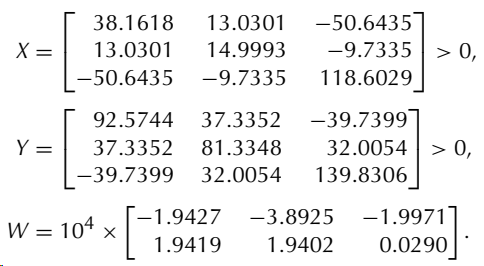
\includegraphics[width=0.7\linewidth]{Solution1/screenshot001}
		\caption[Exercise 1.2.5, Burden-Faires, 8ed.]{}
		\caption{}
		\label{fig:screenshot001}
	\end{figure}
\end{Solution}
 
   
\end{document}